% ===================================================================
%  Week 10 — Session 2: Matching features & rejecting outliers
% ===================================================================
\documentclass[10pt,aspectratio=169]{beamer}
% ===================================================================
%  Shared Beamer preamble for "Practical Image Processing"
%  English slides. Compile with pdfLaTeX.
% ===================================================================

\usetheme{metropolis}
\usepackage[T1]{fontenc}
\usepackage[utf8]{inputenc}
\usepackage{lmodern}
\usepackage{listings}
\usepackage{tcolorbox}
\usepackage{fontawesome5}
\usepackage{booktabs}
\usepackage{amsmath,amssymb}
\usepackage{tikz}
\usepackage{pgfplots}
\pgfplotsset{compat=1.17}
\usetikzlibrary{arrows.meta,positioning,shapes.geometric,fit,backgrounds,matrix}
\tcbuselibrary{skins,breakable}

% ---- Palette --------------------------------------------------------
\definecolor{coursePrimary}{HTML}{1B4965}   % deep blue
\definecolor{courseAccent}{HTML}{E76F51}    % coral
\definecolor{courseGood}{HTML}{2A9D8F}      % teal
\definecolor{courseBad}{HTML}{C0392B}       % red
\definecolor{courseInfo}{HTML}{2980B9}      % blue
\definecolor{codeBg}{HTML}{F5F6FA}
\definecolor{codeKw}{HTML}{8E44AD}
\definecolor{codeStr}{HTML}{2A9D8F}
\definecolor{codeCom}{HTML}{7F8C8D}

\setbeamercolor{frametitle}{bg=coursePrimary}
\setbeamercolor{progress bar}{fg=courseAccent}
\setbeamercolor{alerted text}{fg=courseAccent}
\metroset{block=fill,sectionpage=progressbar,numbering=fraction}

% ---- Code listings (Python is built into listings) -----------------
\lstdefinestyle{course}{
  backgroundcolor=\color{codeBg},
  basicstyle=\ttfamily\scriptsize,
  keywordstyle=\color{codeKw}\bfseries,
  stringstyle=\color{codeStr},
  commentstyle=\color{codeCom}\itshape,
  numberstyle=\tiny\color{codeCom},
  numbers=left, numbersep=6pt,
  showstringspaces=false, breaklines=true, breakatwhitespace=true,
  tabsize=4, columns=fullflexible,
  frame=single, framesep=4pt, rulecolor=\color{gray!30},
  keepspaces=true, upquote=true, language=Python,
}
\lstset{style=course}
\lstdefinelanguage{bash}{
  keywords={cd,pip,python,venv,source,import}, sensitive=true,
  morecomment=[l]{\#}, morestring=[b]', morestring=[b]",
}

% ---- Reusable callout boxes ----------------------------------------
\newtcolorbox{goodbox}[1][Good practice]{colback=courseGood!8,colframe=courseGood,
  fonttitle=\bfseries,title={\faCheck~#1},boxrule=0.6pt,left=4pt,right=4pt,top=3pt,bottom=3pt}
\newtcolorbox{badbox}[1][Pitfall]{colback=courseBad!8,colframe=courseBad,
  fonttitle=\bfseries,title={\faTimes~#1},boxrule=0.6pt,left=4pt,right=4pt,top=3pt,bottom=3pt}
\newtcolorbox{infobox}[1][Note]{colback=courseInfo!8,colframe=courseInfo,
  fonttitle=\bfseries,title={\faInfoCircle~#1},boxrule=0.6pt,left=4pt,right=4pt,top=3pt,bottom=3pt}
\newtcolorbox{mathbox}[1][Math]{colback=coursePrimary!6,colframe=coursePrimary,
  fonttitle=\bfseries,title={\faCalculator~#1},boxrule=0.6pt,left=4pt,right=4pt,top=3pt,bottom=3pt}

\newcommand{\keyidea}[1]{\begin{alertblock}{Key idea}#1\end{alertblock}}
\newcommand{\term}[1]{\textbf{\color{coursePrimary}#1}}
\newcommand{\code}[1]{\lstinline[basicstyle=\ttfamily\small]|#1|}

% ---- A helper to draw a small pixel grid, cells shaded by value ----
% \pixelgrid{ {10,20,120,200,240}, {30,60,130,180,230}, ... }
\newcommand{\pixelgrid}[1]{%
  \begin{tikzpicture}[font=\scriptsize,scale=0.6]
    \foreach \row [count=\ry] in {#1} {
      \foreach \val [count=\cx] in \row {
        \draw[gray,fill=coursePrimary!8] (\cx,-\ry) rectangle ++(1,-1);
        \node at (\cx+0.5,-\ry-0.5) {\val};
      }
    }
  \end{tikzpicture}}


\title{Feature Detection \& Matching}
\subtitle{Week 10 — Session 2: Describing, matching \& rejecting outliers}
\author{Practical Image Processing}
\date{Lecture 10.2 \textbullet\ 60--70 min}

\begin{document}

\maketitle

\begin{frame}{Recap of Session 1}
  \begin{columns}[T]
    \begin{column}{0.6\textwidth}
      \begin{itemize}
        \item Good features are \term{distinctive}, \term{repeatable}, \term{local} — corners fit best.
        \item \term{Harris}: structure matrix $M$, score $R=\det M - k(\mathrm{tr}\,M)^2$; then NMS.
        \item A \term{descriptor} summarizes the patch as an invariant vector.
      \end{itemize}
    \end{column}
    \begin{column}{0.4\textwidth}
      \begin{alertblock}{Today}
        Build the descriptor, \term{match} descriptors across images, and reject the wrong matches —
        then this week's deliverable.
      \end{alertblock}
    \end{column}
  \end{columns}
\end{frame}

\begin{frame}{Roadmap — Session 2}\tableofcontents\end{frame}

% ==================================================================
\section{Building descriptors}
% ==================================================================

\begin{frame}{From keypoint to descriptor vector}
  \begin{itemize}
    \item Take an oriented, scaled patch around the keypoint (from Session 1's detector).
    \item Summarize it as a fixed-length vector so any two keypoints can be compared by distance.
    \item Two families: \term{float} histograms (SIFT) and \term{binary} strings (BRIEF/ORB).
  \end{itemize}
  \keyidea{The descriptor is the ``fingerprint'' of a keypoint. Similar fingerprints $\Rightarrow$ the same physical point.}
\end{frame}

\begin{frame}{SIFT — gradient-orientation histograms}
  \begin{columns}[T]
    \begin{column}{0.52\textwidth}
      \begin{itemize}
        \item Split the patch into a $4\times4$ grid of cells.
        \item In each cell, build an 8-bin histogram of gradient orientations (weighted by magnitude).
        \item Concatenate: $4\times4\times8 = \mathbf{128}$ numbers, then normalize.
      \end{itemize}
    \end{column}
    \begin{column}{0.48\textwidth}
      \begin{center}
      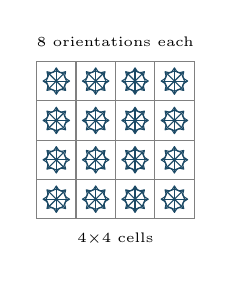
\begin{tikzpicture}[scale=0.5,font=\tiny]
        \draw[step=1,gray] (0,0) grid (4,4);
        \foreach \x in {0.5,1.5,2.5,3.5}
          \foreach \y in {0.5,1.5,2.5,3.5}{
            \foreach \a in {0,45,...,315}
              \draw[coursePrimary,->] (\x,\y)--++(\a:0.35);
          }
        \node at (2,-0.5) {$4{\times}4$ cells};
        \node at (2,4.5) {8 orientations each};
      \end{tikzpicture}
      \end{center}
    \end{column}
  \end{columns}
  \begin{mathbox}
    Orientations are measured \emph{relative} to the keypoint's dominant angle $\Rightarrow$ rotation invariance.
  \end{mathbox}
\end{frame}

\begin{frame}{SIFT — why 128 and why it is robust}
  \begin{itemize}
    \item Histograms tolerate small shifts: a gradient near a cell edge still lands in the right bin-ish.
    \item Normalizing the 128-vector to unit length removes contrast (multiplicative) changes.
    \item Clamping large values then re-normalizing curbs a few dominant gradients (non-linear lighting).
  \end{itemize}
  \begin{goodbox}
    128 floats is a good trade: rich enough to be distinctive, small enough to match fast. This is the
    classic ``gold standard'' descriptor.
  \end{goodbox}
\end{frame}

\begin{frame}{Binary descriptors — BRIEF}
  \begin{columns}[T]
    \begin{column}{0.55\textwidth}
      \begin{itemize}
        \item Pick a fixed pattern of pixel \emph{pairs} inside the patch.
        \item For each pair $(a,b)$: write bit $1$ if $I_a<I_b$, else $0$.
        \item 256 pairs $\rightarrow$ a 256-bit string. Comparing = counting differing bits.
      \end{itemize}
    \end{column}
    \begin{column}{0.45\textwidth}
      \begin{center}
      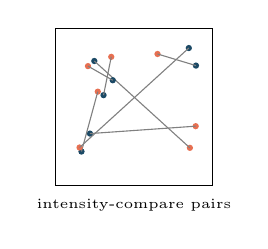
\begin{tikzpicture}[scale=0.5,font=\tiny]
        \draw (0,0) rectangle (4,4);
        \foreach \i in {1,...,7}{
          \pgfmathsetmacro\ax{0.4+3.2*rnd}
          \pgfmathsetmacro\ay{0.4+3.2*rnd}
          \pgfmathsetmacro\bx{0.4+3.2*rnd}
          \pgfmathsetmacro\by{0.4+3.2*rnd}
          \fill[coursePrimary] (\ax,\ay) circle (0.08);
          \fill[courseAccent] (\bx,\by) circle (0.08);
          \draw[gray] (\ax,\ay)--(\bx,\by);
        }
        \node at (2,-0.5) {intensity-compare pairs};
      \end{tikzpicture}
      \end{center}
    \end{column}
  \end{columns}
  \begin{badbox}
    Plain BRIEF is \emph{not} rotation-invariant — rotate the patch and the pairs point elsewhere.
  \end{badbox}
\end{frame}

\begin{frame}{ORB = oriented FAST + rotated BRIEF}
  \begin{itemize}
    \item \term{FAST} keypoints (Session 1) get an orientation from the patch intensity centroid.
    \item BRIEF's sampling pattern is \emph{rotated} by that angle $\rightarrow$ rotation-aware (``rBRIEF'').
    \item Result: a fast, free, rotation-invariant binary descriptor — the practical default.
  \end{itemize}
  \keyidea{ORB gets most of SIFT's robustness at a fraction of the cost, with no patents. Great for real-time.}
\end{frame}

\begin{frame}{SIFT vs ORB (and friends)}
  \begin{center}
  \begin{tabular}{@{}lll@{}}
    \toprule
    \textbf{Descriptor} & \textbf{Type} & \textbf{Note} \\
    \midrule
    SIFT & 128-D float & very robust; the gold standard \\
    SURF & float & faster SIFT-like (patented) \\
    ORB & binary (256-bit) & free, fast, great for real-time \\
    BRIEF & binary & fast but not rotation-invariant alone \\
    \bottomrule
  \end{tabular}
  \end{center}
  \begin{goodbox}
    ORB is the practical default: free, fast, good enough. SIFT when you need maximum robustness.
  \end{goodbox}
\end{frame}

% ==================================================================
\section{Matching descriptors}
% ==================================================================

\begin{frame}{Matching descriptors across images}
  \begin{center}
  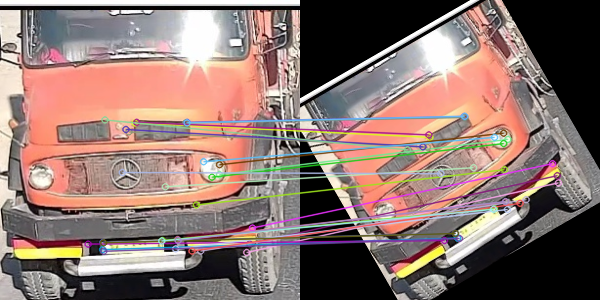
\includegraphics[width=0.9\linewidth]{../assets/matches.png}
  \end{center}
  \vspace{2pt}
  Same car, rotated \& scaled. ORB features still match — lines connect the same physical points.
  This is \term{invariance} working on real data.
\end{frame}

\begin{frame}{How matching works}
  \begin{itemize}
    \item For each descriptor in image A, find the \term{nearest} descriptor in image B (by distance).
    \item Float descriptors (SIFT): \term{Euclidean} distance. Binary (ORB): \term{Hamming} distance.
    \item \term{Brute-force} compares all pairs; \term{FLANN} approximates it fast for large sets.
  \end{itemize}
  \begin{mathbox}
    Hamming distance = number of differing bits — a single fast XOR + popcount for binary descriptors.
  \end{mathbox}
\end{frame}

\begin{frame}{Hamming distance — worked example}
  \begin{columns}[T]
    \begin{column}{0.55\textwidth}
      Two 8-bit ORB descriptors:
      \begin{align*}
        a &= \texttt{1011\,0010}\\
        b &= \texttt{1001\,0110}\\
        a \oplus b &= \texttt{0010\,0100}
      \end{align*}
      Popcount of $a\oplus b = 2$ $\Rightarrow$ Hamming distance $=\mathbf{2}$.
    \end{column}
    \begin{column}{0.45\textwidth}
      \begin{infobox}[Fast in hardware]
        XOR + a single \code{popcount} instruction compares a whole 256-bit descriptor in a few cycles —
        why binary descriptors match so quickly.
      \end{infobox}
    \end{column}
  \end{columns}
\end{frame}

\begin{frame}{Euclidean vs Hamming — pick by descriptor type}
  \begin{center}
  \begin{tabular}{@{}lll@{}}
    \toprule
    \textbf{Descriptor} & \textbf{Distance} & \textbf{OpenCV norm} \\
    \midrule
    SIFT / SURF (float) & Euclidean ($L_2$) & \code{NORM_L2} \\
    ORB / BRIEF (binary) & Hamming & \code{NORM_HAMMING} \\
    \bottomrule
  \end{tabular}
  \end{center}
  \begin{badbox}
    Using \code{NORM_L2} on a binary descriptor (or Hamming on floats) gives garbage matches — match the
    metric to the descriptor.
  \end{badbox}
\end{frame}

\begin{frame}{Brute-force, kNN, and FLANN}
  \begin{itemize}
    \item \term{Brute-force}: compare every A-descriptor to every B-descriptor. Exact, $O(N\!\cdot\!M)$.
    \item \term{kNN match}: return the \emph{two} nearest neighbours per descriptor — needed for the ratio test.
    \item \term{FLANN}: approximate nearest neighbour (kd-trees / LSH). Much faster for thousands of features.
  \end{itemize}
  \keyidea{Small sets: brute-force is fine and exact. Large sets / real-time: FLANN trades a little accuracy for big speed.}
\end{frame}

% ==================================================================
\section{Rejecting bad matches}
% ==================================================================

\begin{frame}{Rejecting bad matches}
  \begin{itemize}
    \item Many nearest-neighbour matches are wrong. Filter them:
    \item \term{Ratio test} (Lowe): keep a match only if the best is much closer than the 2nd-best.
    \item \term{Cross-check}: keep only mutual nearest neighbours.
    \item \term{RANSAC} (Week 11): reject geometric outliers by fitting a transform.
  \end{itemize}
  \begin{badbox}
    Raw matches are noisy. Without the ratio test / RANSAC, a few wrong matches wreck the alignment.
  \end{badbox}
\end{frame}

\begin{frame}{Lowe's ratio test — worked example}
  For a descriptor in A, its two nearest neighbours in B have distances $d_1$ (best), $d_2$ (2nd):
  \[ \text{keep if } \frac{d_1}{d_2} < 0.75 . \]
  \begin{columns}[T]
    \begin{column}{0.5\textwidth}
      \begin{goodbox}[Distinctive — keep]
        $d_1=30,\ d_2=90$: ratio $=0.33<0.75$. The best is clearly better $\Rightarrow$ trust it.
      \end{goodbox}
    \end{column}
    \begin{column}{0.5\textwidth}
      \begin{badbox}[Ambiguous — reject]
        $d_1=80,\ d_2=88$: ratio $=0.91>0.75$. Two candidates almost tie $\Rightarrow$ unreliable, drop it.
      \end{badbox}
    \end{column}
  \end{columns}
  \keyidea{The ratio test asks ``is this match \emph{uniquely} good?'' — it kills matches in repetitive texture.}
\end{frame}

\begin{frame}{Cross-check — mutual nearest neighbours}
  \begin{columns}[T]
    \begin{column}{0.55\textwidth}
      \begin{itemize}
        \item A's best match in B is $b$; B's best match for $b$ back in A must be the same $a$.
        \item Only \emph{mutual} best matches survive — a cheap, symmetric filter.
        \item OpenCV: \code{BFMatcher(..., crossCheck=True)} (do not combine with the ratio test).
      \end{itemize}
    \end{column}
    \begin{column}{0.45\textwidth}
      \begin{center}
      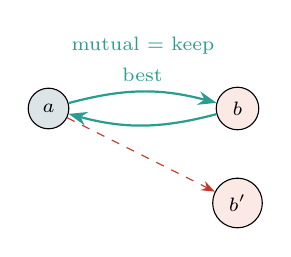
\begin{tikzpicture}[font=\scriptsize,>=Stealth]
        \node[circle,draw,fill=coursePrimary!15] (a) at (0,1) {$a$};
        \node[circle,draw,fill=courseAccent!15] (b) at (2.4,1) {$b$};
        \node[circle,draw,fill=courseAccent!15] (c) at (2.4,-0.2) {$b'$};
        \draw[->,courseGood,thick] (a) to[bend left=15] node[above]{best} (b);
        \draw[->,courseGood,thick] (b) to[bend left=15] (a);
        \draw[->,courseBad,dashed] (a) -- (c);
        \node[courseGood] at (1.2,1.8) {mutual = keep};
      \end{tikzpicture}
      \end{center}
    \end{column}
  \end{columns}
\end{frame}

\begin{frame}{RANSAC — a one-slide preview (Week 11)}
  \begin{itemize}
    \item Even after ratio/cross-check, some geometric outliers remain.
    \item \term{RANSAC}: repeatedly pick a minimal random sample, fit a transform, count \term{inliers}
          (matches that agree with it), keep the best-supported model.
    \item The consensus transform (a homography) both filters outliers \emph{and} aligns the images.
  \end{itemize}
  \keyidea{Ratio test / cross-check clean up \emph{descriptor} errors; RANSAC cleans up \emph{geometry} errors. You need both.}
\end{frame}

% ==================================================================
\section{Scale invariance \& applications}
% ==================================================================

\begin{frame}{Scale invariance: the pyramid}
  \begin{columns}[T]
    \begin{column}{0.55\textwidth}
      \begin{itemize}
        \item To find features at any size, build an \term{image pyramid} (progressively smaller copies).
        \item Detect at each level; the scale where a feature is strongest is its ``characteristic scale.''
        \item That is how SIFT/ORB match a small template to a large photo.
      \end{itemize}
    \end{column}
    \begin{column}{0.45\textwidth}
      \begin{center}
      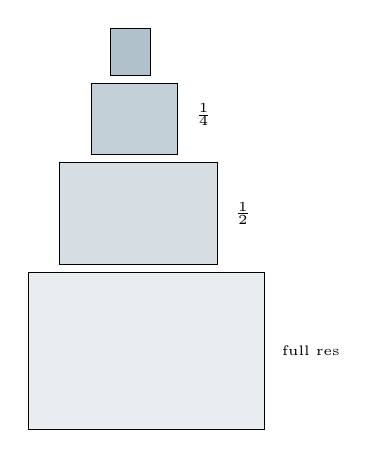
\begin{tikzpicture}[font=\tiny]
        \draw[fill=coursePrimary!10] (0,0) rectangle (3,2);
        \draw[fill=coursePrimary!18] (0.4,2.1) rectangle (2.4,3.4);
        \draw[fill=coursePrimary!26] (0.8,3.5) rectangle (1.9,4.4);
        \draw[fill=coursePrimary!34] (1.05,4.5) rectangle (1.55,5.1);
        \node[right] at (3.1,1) {full res};
        \node[right] at (2.5,2.75) {$\tfrac12$};
        \node[right] at (2.0,4.0) {$\tfrac14$};
      \end{tikzpicture}
      \end{center}
    \end{column}
  \end{columns}
\end{frame}

\begin{frame}{How many matches do you need?}
  \begin{itemize}
    \item To estimate a \term{homography} (Week 11) you need $\geq 4$ good correspondences.
    \item In practice, gather dozens of matches, then let \term{RANSAC} pick a consistent set of 4+.
    \item More good matches $\rightarrow$ a more stable, accurate transform.
  \end{itemize}
  \keyidea{Quantity gives robustness: many matches let outlier rejection succeed even when a third are wrong.}
\end{frame}

\begin{frame}{Applications of features}
  \begin{itemize}
    \item \term{Image stitching} (panoramas): match features, find the transform, blend.
    \item \term{Object recognition}: match a template's features to a scene.
    \item \term{Tracking, SLAM, AR}: follow features across video to estimate motion.
    \item \term{DocScan}: match the page/template to align and rectify (Week 11).
  \end{itemize}
\end{frame}

\begin{frame}{Classical features vs deep features}
  \begin{itemize}
    \item Classical (SIFT/ORB): hand-designed, interpretable, no training — still excellent for geometry.
    \item Deep (learned descriptors, SuperPoint): better under extreme appearance change, need training.
    \item For alignment/geometry, classical features remain a strong, practical choice.
  \end{itemize}
  \keyidea{Features are how a computer says ``this point here is the same as that point there'' — the foundation of geometric vision.}
\end{frame}

% ==================================================================
\section{In-class exercise}
% ==================================================================

\begin{frame}{\faPen~In-class exercise (10 min)}
  \begin{infobox}[Reason about matching]
  \end{infobox}
  \begin{enumerate}
    \item Two ORB descriptors: \texttt{1100\,1010} and \texttt{1110\,0011}. Hamming distance?
    \item A match has $d_1=60,\ d_2=66$. Does Lowe's ratio test (0.75) keep it? Why?
    \item You match a template plate to a photo taken at an angle and half the size. Which
          descriptor properties make this possible?
  \end{enumerate}
\end{frame}

\begin{frame}{\faPen~Debrief}
  \begin{itemize}
    \item (1) XOR $=\texttt{0010\,1001}$, popcount $=3 \Rightarrow$ Hamming distance $\mathbf{3}$.
    \item (2) Ratio $=60/66=0.91>0.75 \Rightarrow$ \term{reject} — the two candidates nearly tie, so it is ambiguous.
    \item (3) \term{Scale and rotation invariance} — the descriptor is the same despite size/angle change.
  \end{itemize}
  \keyidea{Good features + good matches + outlier rejection = reliable correspondence, the basis of alignment.}
\end{frame}

% ==================================================================
\section{Wrap-up \& deliverable}
% ==================================================================

\begin{frame}[fragile]{Features in code}
\begin{lstlisting}[language=Python]
orb = cv2.ORB_create(500)
kp1, des1 = orb.detectAndCompute(img1, None)
kp2, des2 = orb.detectAndCompute(img2, None)
bf = cv2.BFMatcher(cv2.NORM_HAMMING, crossCheck=True)
matches = sorted(bf.match(des1, des2), key=lambda m: m.distance)
# next week: cv2.findHomography(pts1, pts2, cv2.RANSAC) to align
\end{lstlisting}
  Detect $\rightarrow$ describe $\rightarrow$ match $\rightarrow$ (Week 11) estimate the transform.
\end{frame}

\begin{frame}[fragile]{Matching with the ratio test}
\begin{lstlisting}[language=Python]
bf = cv2.BFMatcher(cv2.NORM_HAMMING)          # no crossCheck for kNN
knn = bf.knnMatch(des1, des2, k=2)            # 2 nearest per descriptor
good = [m for m, n in knn if m.distance < 0.75 * n.distance]
print(len(good), "good matches after Lowe's ratio test")
\end{lstlisting}
  \begin{goodbox}
    Use \code{knnMatch} + ratio test \emph{or} \code{crossCheck=True} — not both at once.
  \end{goodbox}
\end{frame}

\begin{frame}{What you should now be able to do}
  \begin{itemize}
    \item Explain how SIFT and ORB build their descriptor vectors.
    \item Match descriptors with the right metric (Euclidean vs Hamming), brute-force or FLANN.
    \item Reject bad matches with the ratio test and cross-check; explain RANSAC's role.
    \item Connect scale/rotation invariance to real matching across views.
  \end{itemize}
\end{frame}

\begin{frame}{This week's deliverable}
  \begin{alertblock}{Due before Week 11 (see \code{project/})}
    \begin{enumerate}
      \item Detect Harris corners and ORB keypoints on real images; visualize.
      \item Match ORB features between an image and a rotated/scaled copy; count good matches.
      \item Apply the ratio test / cross-check; show how it removes wrong matches.
      \item Note: how will feature matching help align a photographed page in DocScan?
    \end{enumerate}
  \end{alertblock}
\end{frame}

\begin{frame}[standout]
  Features are ``the same point, seen again.''\\[4pt]
  \normalsize Detect distinctive points, describe them invariantly, match across images, reject outliers.
\end{frame}

\end{document}
